\setchapterpreamble[o]{%
  \dictum[Steve Jobs]{\textit{``Design is not  just what it looks like and
      feels like. Design is how it works.''}}}

\chapter{Design and Implementation}
\label{cha:design}

This chapter is about the design and implementation of the \emph{Xen-Based
  Execution  Environment} (\gls{glo:XenBEE}).   The  execution environment
incorporates  a total  of three  main  components: the  \emph{xbe} on  the
user's side, the \emph{xbed} on  the server's side and the \emph{xbeinstd}
on  the  side of  a  single virtual  machine.   All  components have  been
implemented     using    the     \emph{Python}     programming    language
\cite{python-language}. In particular, version  $2.5$ of that language has
been used.

Some additional  modules and programs, that  are not part  of the standard
libraries shipped with Python, have been used, though. Among these are for
instance  the \texttt{twisted}  framework \cite{twisted-python}  which has
been  used  for  the  network  code,  a  library  called  \texttt{libvirt}
\cite{libvirt}  that  was used  to  connect  to  the Xen  virtual  machine
monitor, and a library that  provides Python bindings to the \texttt{curl}
library \cite{pycurl}.


\section{Overview}
\label{sec:design:overview}

The picture in Figure~\ref{fig:architecture-overview} shows an overview of
the three components which, when put together, make up the \emph{Xen-Based
  Execution Environment} (\gls{glo:XenBEE}).

\begin{figure}[ht]
  \centering
  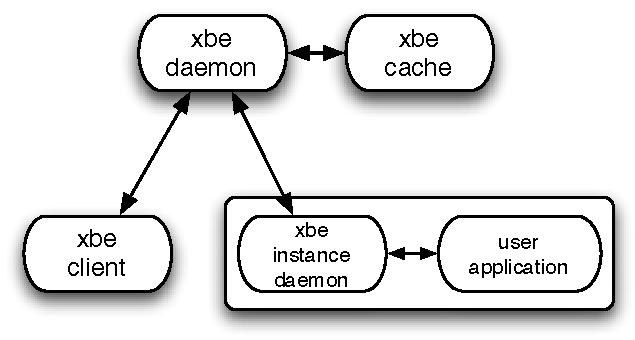
\includegraphics[scale=.7]{architecture-overview}
  \caption[Overview of the  \gls{glo:XenBEE} components]{The components of
    the Xen-Based Execution Environment}
  \label{fig:architecture-overview}
\end{figure}

On the left hand side of the picture are the users using the \emph{xbe} to
communicate with the execution  environment. The \emph{xbe} refers in this
case  to the command  line tool  which I  have implemented  as a  proof of
concept  to interact  with the  \emph{xbed}.  The  interface that  an user
utilizes to execute his applications  with the \gls{glo:XenBEE} could be a
web-portal or some other tool with a graphical user interface, as well.

\medskip

On the right hand side are the components that are required to execute the
applications within  virtual machines.  The \emph{xbed} has  to be running
on a machine, that supports  the Xen hypervisor.  It maintains an internal
connection to  a local  cache, which can  be used  by any user  to deposit
arbitrary data on the  server side.  The \emph{xbed} uses \texttt{libvirt}
to connect to the Xen hypervisor and to manage active virtual machines.

Each virtual machine  must provide the \emph{xbeinstd}, that  means it has
to be started at some point during the initialization process of the guest
operating system. Any image that is submitted to the execution environment
must therefore  contain this  program. The \emph{xbeinstd}  is responsible
for two  major issues:  executing the actual  application and  keeping the
virtual machine instance alive.   Execution of an application involves for
instance  passing  arguments  to   the  executable,  setting  the  working
directory and redirecting the input and output streams. The \emph{xbed} is
going  to shut  stale virtual  machines down,  unless  the \emph{xbeinstd}
sends  regular keep-alive  messages  to the  \emph{xbed}.   If the  user's
application has finished, the \emph{xbeinstd} signals the \emph{xbed} that
the virtual machine is ready to be shut down.

\medskip

The  thicker connections  between \emph{xbe}  and \emph{xbed}  as  well as
between \emph{xbed}  and \emph{xbeinstd} are  logical connections realized
by using message-queues and one  or more \gls{glo:MQS} in between. Whereas
he  thinner links  are either  inner-process connections  (in case  of the
cache) or  connections between  parent and child  process (in case  of the
user-application).

\section[The Xen-Based Execution Daemon]{The Xen-Based Execution Daemon (xbed)}
\label{sec:xbed}

This  section describes  the  ``heart'' of  the  \gls{glo:XenBEE} ---  the
\emph{xbed}.   The  \emph{xbed}  is  itself composed  of  several  smaller
components that  are each responsible for  a single detail  of the daemon.
The    main    components    though    are   the    \texttt{Cache},    the
\texttt{TaskManager}  and the  \texttt{InstanceManager}. The  former  is a
rather simple implementation of a local data cache, that will be discussed
in a later section.

\begin{figure}[ht]
  \centering
  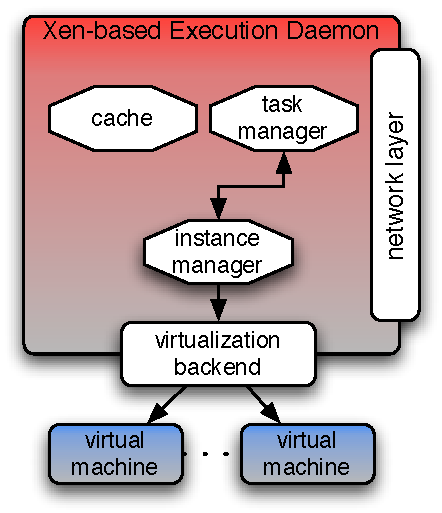
\includegraphics[scale=.55]{xbed-architecture}
  \caption[Components of the xbed]{The most important components of the xbed}
  \label{fig:xbed-architecture}
\end{figure}

\subsubsection{Network Layer}

On startup, the  daemon tries to connect to  the message-queue server that
has been  defined either in  its configuration file  or as a  command line
parameter. This process  is realized by the \emph{network  layer}. It uses
the  \texttt{twisted} framework to  establish a  \gls{glo:TCP} connection.
When the connection has been successfully established, a special transport
protocol --- the  STOMP protocol --- is attached  to the connection. STOMP
is  the \emph{Streaming  Text Oriented  Messaging Protocol}  and basically
defines a  very simple protocol to  send and receive text  messages over a
message-queue server.  On top of  this text message based protocol are XML
based  protocols  that  accomplish  the whole  communication  between  all
components.   There is currently  a basic  XML protocol  that encapsulates
single ``messages'', consisting just of header and body, and two protocols
that  connect up  the \emph{xbe}  and the  \emph{xbeinst}  accordingly.  A
special  protocol providing  security  related services  (\ie privacy  and
validity) can be added as an additional layer.

Anyway, the  details of the \gls{glo:STOMP}  and XML protocols  as well as
the network layer,  which is to some extent equal  among all components of
the        \gls{glo:XenBEE},       will       be        discussed       in
Section~\ref{sec:communication-protocol},
\emph{\nameref{sec:communication-protocol}}.

\subsubsection{Task-Manager}

When an  user submits,  terminates or  requests the status  of one  of her
jobs, the  message is actually handled by  the \texttt{TaskManager}.  This
component controls all tasks, the system knows of. A ``task'' does in this
case  not refer  to the  actual application  an user  submitted, but  to a
container that holds the task's  state machine, description and probably a
reference to the virtual machine instance used for this task.

A new task gets initialized every  time an user requests a reservation. At
this time it contains nothing more  than the state machine which is in its
start-state                               (\ie \texttt{Pending:Reserved}).
Section~\ref{sec:xbed:job-model}  discusses   the  implementation  of  the
job-model that has been used to  represent an activity.

Each task and each reservation has its own unique identifier by which they
are known  to the system  and to the  user.  Those unique  identifiers are
implemented     by    using     \emph{Universal     Unique    Identifiers}
(\gls{glo:UUID}s).  Whereas  the task identifier is more  or less publicly
available\footnote{a listing  of all current tasks comparable  to the UNIX
  \texttt{ps}  command could be  possible}, the  identifier of  the user's
reservation is  only known to  that particular user (or  some intermediary
software such as  a Calana-agent). All requests that an  user makes to the
system,  that refer  to a  reservation and  hence to  a task,  require the
reservation's unique identifier.

When an user confirms a reservation,  he also sends the job description as
a \gls{glo:JSDL}  document along with the confirmation  message.  The task
is  thus completely  specified and  may  perform the  transition into  the
\texttt{Executing} state. To this time, the task-manager creates a special
spool directory  for that  task which is  eventually going to  contain all
necessary  files to  create the  virtual  machine and  execute the  user's
application. The  details of how the  required files are  obtained will be
discussed  in   a  later  section  (Section~\ref{sec:xbed:data-transfer}).
After  all   files  have  been   retrieved,  the  \texttt{InstanceManager}
component is used to create a new virtual machine for the task.

\subsubsection{Instance-Manager}

The instance-manager's purpose is  to create, control, monitor and destroy
active virtual  machine instances.  Again  unique identifiers are  used to
name the  virtual machines. To start  a virtual machine  several files are
required:  an   operating  system  installation  residing   in  a  special
file-system  \gls{glo:image} file, a  \gls{glo:kernel} and  potentially an
initial ramdisk  image (initrd),  that contains additional  device drivers
and setup  routines that  are not directly  included in the  kernel. Those
files must  be provided by  the user,  since he is  the one who  knows his
application and how the operating  system has to be configured to actually
execute the application.

By just using these three files, a virtual machine cannot be created right
away, it must be \emph{configured}  first.  The configuration of a virtual
machine  is manifold,  it contains  descriptions of  the  operating system
which shall be used (\ie  the mentioned three files), memory settings (\ie
the amount  of virtualized physical  memory), them number of  virtual CPUs
and network parameters.

\subparagraph{Instance Configuration and Setup}

The \emph{xbed}  provides the possibility to  use different virtualization
back-ends,  but  the  current  implementation supports  only  Xen  virtual
machines. It could, for instance, be possible to implement a back-end that
uses VMWare's  \cite{vmware} virtual machines, even no  virtual machine at
all could be thinkable.

The back-end uses  the \texttt{libvirt} \gls{glo:API} to connect
to  the Xen hypervisor.  This connection  is basically  used to  query the
current state of  a virtual machine and to shut  a running virtual machine
down.   Virtual machine creation  is implemented  by using  a call  to the
\texttt{xm} command line tool provided by the Xen user-space tools.  Prior
a  new  instance   can  be  created,  a  configuration   file  has  to  be
generated. This configuration file contains the mentioned parameters.

The  network  configuration   of  a  virtual  machine  is   based  on  the
\emph{Dynamic Host Configuration  Protocol} (\gls{glo:DHCP}).  That means,
the guest  \gls{glo:OS} has  to be configured  to use  \gls{glo:DHCP}. The
administrator of  the host, on which  the \emph{xbed} runs,  can specify a
list  of  \gls{glo:MAC}  addresses  that  shall be  used  by  the  virtual
machines. In addition to  these \gls{glo:MAC} addresses, the administrator
can also  specify a \gls{glo:URI}  or an IP  address by which  the virtual
machine

Virtualized  physical  memory  and  the  number of  virtual  CPUs  can  be
specified  in the  \gls{glo:JSDL} document  using the  predefined resource
descriptions.

\subparagraph{Instance Creation}

The next step is the generation  of a configuration file which can be used
by the back-end --- in this case  Xen --- to set up a new virtual machine.
The task's  state machine  is triggered  to change its  state to  the next
sub-state   of  \texttt{Running}:  \texttt{InstanceStarting}.    Once  the
virtual machine has  been created, the \emph{xbed} awaits  a callback from
the virtual machine.  This scallback expresses itself in form of a message
sent  by  the \emph{xbeinstd}  running  within  the  just created  virtual
machine.  If  this signal does  not get sent  within a given  timeout, the
virtual  machine instance  is assumed  to  be broken  and is  going to  be
destroyed, resulting in a failed  execution of the user's task, of course.
This callback fulfills two important functions --- it makes sure, that the
virtual machine's  network configuration is correct  and fully functional,
and  that the  \emph{xbeinstd}  did start  properly  --- thus,  improperly
configured images are recognized very fast.  Now, that the virtual machine
is ready to execute the  user's application, the task's description may be
sent to  the \emph{xbeinstd} and  the task's state machine  may eventually
change  its state  to  \texttt{Executing}. The  details  of executing  the
application is going to be discussed in Section~\ref{sec:xbeinstd}.

After  finishing the  execution  of the  user's  application, the  virtual
machine will  be shut down and the  result can be staged  out according to
the specified \gls{glo:JSDL} document.

\bigskip

The next sections  describe the implementation of the  used job-model, how
the staging  of input  and output data  is performed  and how an  user can
benefit from using the provided data-cache.

\subsection{Job-model Implementation}
\label{sec:xbed:job-model}

In     the     sections    \emph{`\nameref{sec:fundamentals:bes}'}     and
\emph{`\nameref{sec:calana-support}'}               on               pages
\pageref{sec:fundamentals:bes}       and      \pageref{sec:calana-support}
respectively, I have already discussed the usage of the job-model that has
been  proposed  by the  \gls{glo:OGSA}-\gls{glo:BES}  working group.   The
Calana  architecture   requires  the  model  to   contain  extensions  for
\emph{reservation} and \emph{data staging}.

To model  the process of starting  a virtual machine, I  have extended the
model  again  to provide  an  additional state  \texttt{Instance-Starting}
which  is a  sub-state  of  the basic  state  \texttt{Running}. The  final
job-model is shown in Figure~\ref{fig:bes-job-model}.

\begin{figure}[ht]
  \centering
  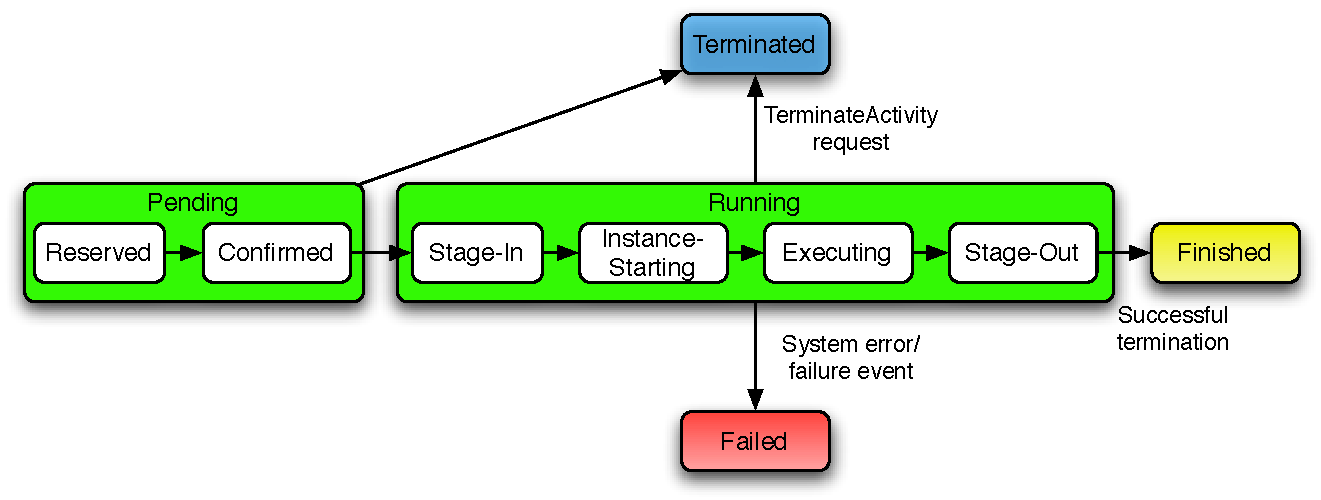
\includegraphics[scale=.55]{bes-job-model}
  \caption{The job-model used in the \gls{glo:XenBEE}}
  \label{fig:bes-job-model}
\end{figure}

The  implementation of  this model  builds up  on an  implementation  of a
\emph{Finite State  Machine} (\gls{glo:FSM}).  The  \texttt{Task} class, I
mentioned  earlier,  contains  a  reference  to an  instance  of  such  an
\gls{glo:FSM}. Each time  a state change is desired,  the \gls{glo:FSM} is
called with  an ``input'' signal. The \gls{glo:FSM}  then calls registered
functions that  implement the transition's  behavior. If, for  example, an
user wants to terminate his  activity, the \gls{glo:FSM} is presented with
a ``terminate-token''. The FSM  calls then specialized functions that deal
with the termination  request according to the current  state. That means,
distinct   functions    are   perhaps   called    when   traversing   from
\texttt{Pending:Reserved}    and    \texttt{Running:Executing}   to    the
\texttt{Terminated} state, respectively.

Some of the transitions  involve rather complex and time-consuming actions
(\eg file  transfers).   Those  complex  transitions are  represented  by
\emph{activity-objects}.    An   activity-object   is  an   object,   that
encapsulates  some behavior  along  with  a state  ---  commonly known  as
\emph{Function}-objects or \emph{Functors}.  I named them activity-objects
on  purpose, because they  are usually  executed by  a separate  thread of
control  in concurrency  to other  activities within  the  system. Another
reason for  encapsulating some of  the transitions in  activity-objects is
the possible intervention by an user.

The BES  model allows an  user to terminate  his activity at any  time. In
particular that means,  that any action belonging to  that activity, which
currently takes place  on the server, has to be  stopped or aborted.

Since the task-manager does not only create, but also manage the tasks, he
is responsible for stopping current activities of a task if he is asked to
do so.  For that reason, he is  in charge of a per task list that contains
all current activities  for that task. If the task-manage  is now going to
handle a request for termination of one of the tasks, he first cancels all
registered activity-objects before letting the task to change its state to
\texttt{Terminated}.

\begin{figure}[ht]
  \centering
  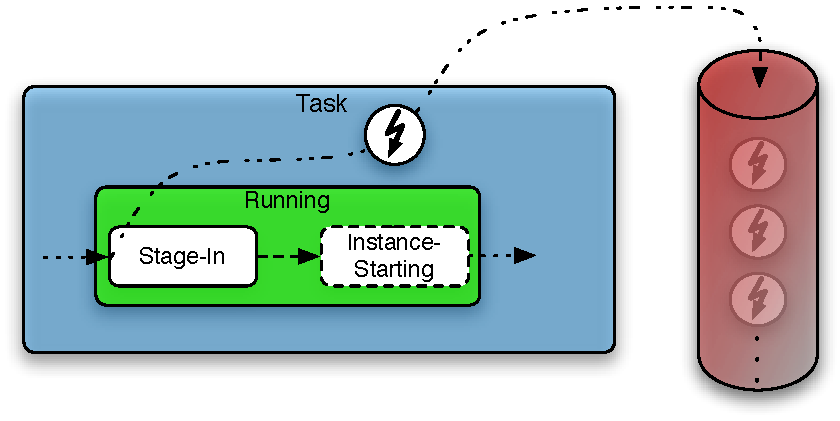
\includegraphics[scale=.55]{activity-queue}
  \caption{Handling of \emph{activity-objects} with an activity-queue.}
  \label{fig:activity-queue}
\end{figure}

The picture in Figure~\ref{fig:activity-queue} shows such an occasion. The
task (represented by  the blue box) is currently  in the \texttt{Stage-In}
sub-state  of \texttt{Running}  and is  awaiting the  availability  of its
required  files.  The  activity  which represents  here  the operation  of
staging files in is shown as  the encircled lightning bolt.  When the task
transitions  into  the \texttt{Stage-In}  state,  it  registers the  shown
activity with  the task-manager. The task-manager  in turn adds  it to his
queue of current activities (shown as the reddish tube in the right of the
picture).  When  the activity is  finished (figuratively speaking:  if the
activity exits through  the bottom of the tube), the  task may advance its
state to \texttt{Instance-Starting}, \ie it  can be attempted to start an
instance for this task.

Since  the  retrieval of  files  from  different  locations (specified  by
\gls{glo:URI}s  in the \gls{glo:JSDL})  may take  some time,  this example
also motivates  the usage of threads  to decouple other  activities of the
system  from these  steps. When  terminating  an activity,  the thread  is
signalled to abort whatever it is doing at the time.

\bigskip

The  whole   cycle  through   which  a  task   may  run  is   depicted  in
Figure~\ref{fig:act-execute-task}  as  an   activity  diagram.   The  only
sub-activity that  cannot be  aborted at all  is the  \emph{stop instance}
operation. That is because the  shutdown process of the underlying virtual
machine just cannot  be cancelled or reversed. That is  also the reason to
not having an extra sub-state for that operation in the job-model.

The  process starts  with waiting  on  a ``ready-to-go''  signal, that  is
usually included  directly in the \texttt{Confirm} message  received by an
user,  but  can  also  be  given  in  a  subsequent  message  on  its  own
(\texttt{Start\-Activity})\footnote{the  communication  protocol  and  the
  messages           involved          are           discussed          in
  Section~\ref{sec:communication-protocol},
  \emph{\nameref{sec:communication-protocol}}.}.  The  next steps resemble
the previously discussed job-model. Of course, any of those activities may
\emph{fail}, which effectively  results in the failing of  the whole task.
The operations that are involved  when one of the sub-activities fails are
the  same  as  for  the  abortion of  that  sub-activity.   Actually,  the
\emph{stop  instance}  operation  cannot  fail  either,  since  it  always
possible to forcibly shut a virtual machine down.

\begin{figure}[ht]
  \centering
  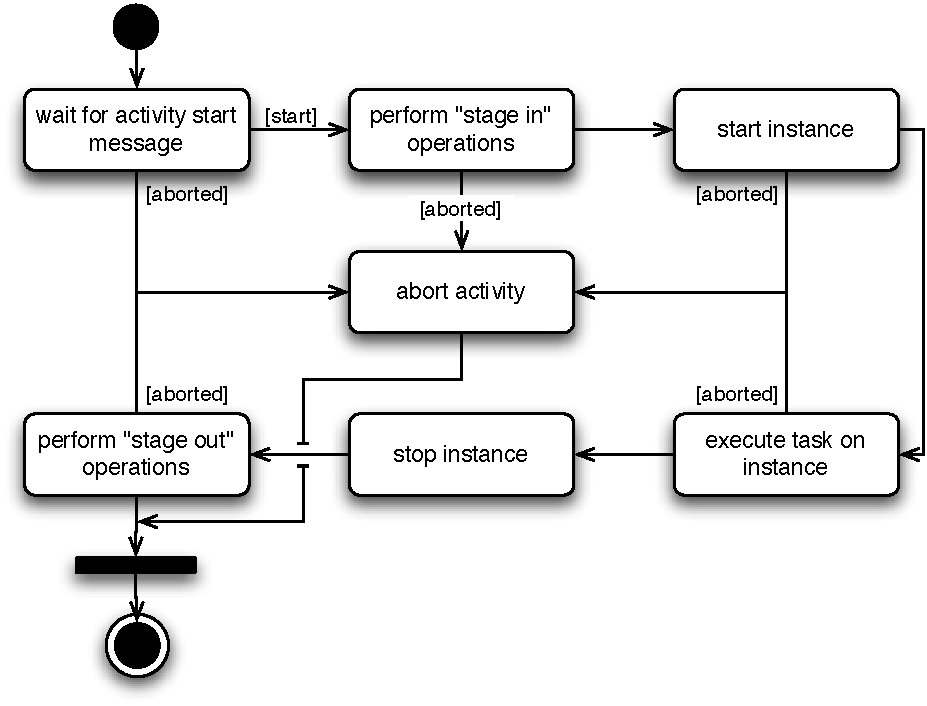
\includegraphics[scale=.55]{act-execute-task}
  \caption[Summary of executing a task]{Summary of the steps involved when executing a task.}
  \label{fig:act-execute-task}
\end{figure}

The \emph{start  instance} operation differs from the  other operations in
that two components are involved, the \emph{xbed} and the \emph{xbeinstd}.
The \emph{xbed}  first attempts  to start a  back-end instance (\eg  a Xen
virtual machine) and waits for the instance to be started, eventually.

After the instance  has been started, \ie the back-end  did not reject the
provided  configuration, the  \emph{xbed}, actually  the  thread executing
this  particular  activity,  waits  for  the \emph{xbeinstd}  to  send  an
\texttt{Instance\-Available}        message       back        to       the
\emph{xbed}. Figure~\ref{fig:act-start-instance} shows the details of that
particular activity.

\begin{figure}[ht]
  \centering
  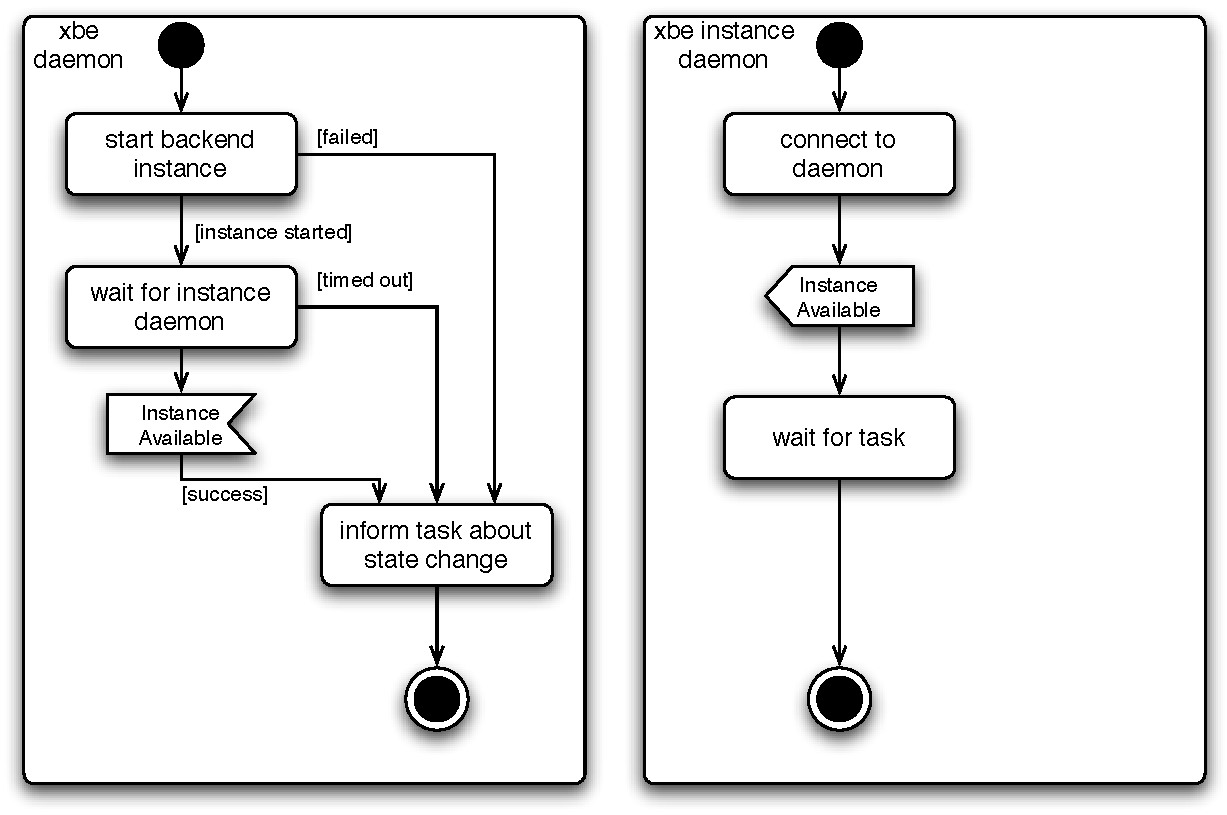
\includegraphics[scale=.55]{act-start-instance}
  \caption[Start Instance Activity]{The  \emph{xbed} waits for the virtual
    machine to  be available.   The availability of  a virtual  machine is
    made sure by waiting on a special message from the \emph{xbeinstd}.}
  \label{fig:act-start-instance}
\end{figure}


As you can see, there are  three different outcomes for this activity. The
instance can  be flagged as  available, which renders the  task eventually
executable,  the activity  can as  well be  aborted due  to a  request for
termination by  the user, or  the instance can  fail to start at  all. The
task's state will be changed according to the outcome of this activity.

After   sending   the   \texttt{Instance\-Alive}   notification   to   the
\emph{xbed},  the  \emph{xbeinstd}   waits  for  the  task's  description.
Additionally,  it will send  messages to  the \emph{xbed}  regularly, thus
making sure, that the virtual machine is still ``alive''.

\bigskip

The  next section deals  with the  staging operations  in more  detail. In
particular that means, how exactly  the files are retrieved, how files can
be compressed  to reduce  the required network-bandwidth  and how  one can
make sure that the file has been transfered correctly.

\subsection{Data Transfer Handling}
\label{sec:xbed:data-transfer}

The  handling  of data  transfer  covers the  staging  of  files into  the
execution environment and out from the execution environment, in this work
referred   to  as  ``stage-in''   and  ``stage-out''   respectively.   The
description  that  is  required  for  each of  the  staging  processes  is
completely  covered  within  the  \gls{glo:JSDL} document,  that  an  user
submitted  to the  execution  environment.  However,  some extensions  are
required,       those       will       be      handled       with       in
Section~\ref{sec:xen-based-submission}.

The  stage-in process  is  twofold.  The  first  part of  stage-in is  the
acquirement of files  that are mandatory for the  execution environment to
create    virtual    machine,    these    are    the    early    mentioned
\emph{\gls{glo:image}}  and  \emph{\gls{glo:kernel}}  files  (probably  an
\emph{\gls{glo:initrd}},  as well).   Without these  files, the  next part
cannot be started.

The second  part of the stage-in  process handles the input  files that an
user had specified for his application. These definitions use the standard
\texttt{DataStaging}  element of  the \gls{glo:JSDL}  specification. These
files  are directly  retrieved into  the virtual  machine image,  that was
previously obtained, hence the two parts of the staging process.

All files, including the virtual machine specific ones, are referred to as
\emph{Uniform  Resource  Identifier}s  (\gls{glo:URI}s). That  means,  all
files must be ``somehow'' accessible by the \emph{xbed}.  An user can, for
instance, specify files that  are located on an \texttt{\gls{glo:HTTP}} or
on an \texttt{\gls{glo:FTP}} server --- currently only these two protocols
and  a special  URI to  reference to  cached files  are  supported.  Those
\gls{glo:URI}s are then retrieved by the \emph{xbed} by using the standard
mechanisms for  file retrieval  based on these  protocols ---  the library
\texttt{libcurl}, which relates to the UNIX \texttt{curl} command, is used
to implement download and upload.

\subsubsection{Support for compressed files}

As said before,  all input files related to  the application are retrieved
into  the virtual  machine image  directly. Consequently,  the  image must
provide enough  free space  to hold all  input and generated  output data,
which  can be  quite a  lot. Since  the  image is  an ordinary  file on  a
file-system, it can  easily consume unpredictable size. This  image has to
be  transfered  from  the user  (\ie  the  location  he specified  in  the
\gls{glo:JSDL}) to  the host on  which the \emph{xbed}  runs. Fortunately,
the image is nearly empty before transmitting it, since it contains only a
basic operating system installation  along with the user's application and
its dependencies.

The \emph{xbed} allows an user to submit compressed files. The compression
is extremely  useful when the file is  mostly ``empty'' as it  is the case
for the  image files, for  instance --- an  image file that was  $8$~GB in
size and contained  about $750$~MB data produced a  compressed file (using
\texttt{bzip2})  that was  about  $500$~MB  in size  only.   The usage  of
compressed files  reduces the  time needed to  transfer large,  but mostly
empty images significantly. The user is allowed to tag every file that she
submits to the execution environment  with the mode of compression and the
\emph{xbed} will decompress the file after retrieval.

\begin{figure}[ht]
  \centering
  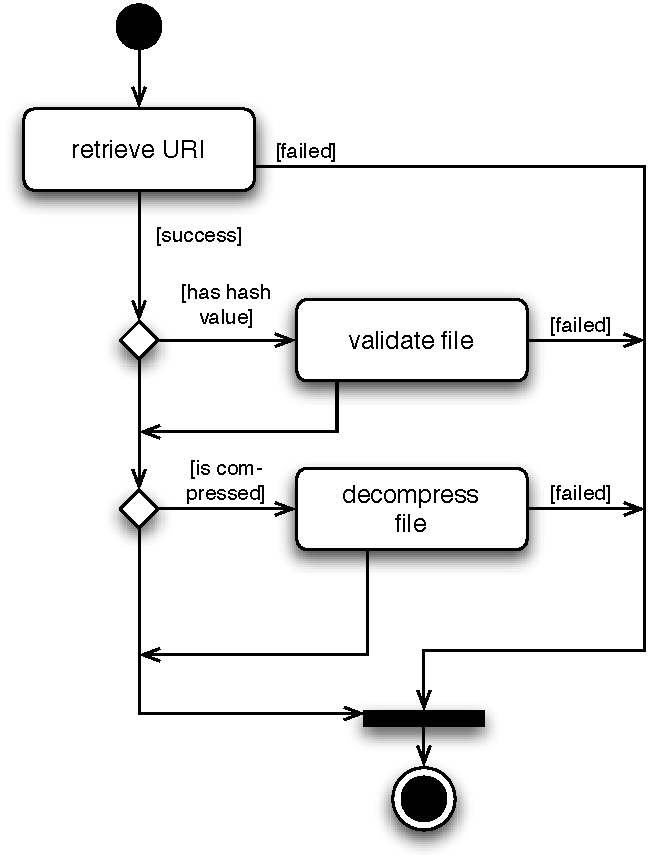
\includegraphics[scale=.55]{act-retrieve-file}
  \caption[File  Retrieval  Activity]{Steps  involved when  retrieving  a
    \gls{glo:URI}.}
  \label{fig:act-retrieve-file}
\end{figure}

\subsubsection{Support for validation of files}

Figure~\ref{fig:act-retrieve-file} shows the involved steps when a file is
retrieved by the \emph{xbed}. Another feature added to this process is the
validation of the retrieved data. If  an user wants to make sure, that the
file had not been modified in some way, she can provide a checksum and the
used    algorithm   along   with    the   \gls{glo:URI}.     Typically   a
\emph{cryptographic  hash   function}  is   used  to  compute   a  digital
fingerprint of the  data. All secure hash algorithms  that are provided by
the  Python  \texttt{hashlib} module  are  supported  (some examples  are:
\texttt{SHA1}, \texttt{SHA256}, \texttt{MD5}).

\subsubsection{The whole stage-in process}

The  stage-in   process  is   split  into  several   steps  as   shown  in
Figure~\ref{fig:act-stage-in}. The process always starts with the creation
of a \texttt{\gls{glo:chroot}} environment\footnote{The terms \emph{chroot
    environment}  and \emph{jail  environment} are  used interchangeably.}
within  the spool  directory that  has been  created for  that  task.  The
description of the  necessary files for a virtual  machine is contained in
an extra element within the task's \gls{glo:JSDL} description. An user can
either specify the required files (image, kernel and initrd) on its own or
he can specify a  \texttt{bzip2} compressed tar archive (``package'') that
contains these files.  Additionally, an user has the possibility to define
several executable scripts that  are uploaded to the execution environment
and get called at various stages of the stage-in process.

After  the package  or  the  virtual machine  files  have been  retrieved,
validated and  probably decompressed, the ``pre-setup''  hook is executed.
This  hook consists  of the  scripts that  were either  in the  package or
specified  by the user  and tagged  to be  in this  hook. All  scripts are
executed in the previously created \gls{glo:chrootenv} so that they cannot
access any file that does not belong to this task. Until now the execution
environment had  not touched the  image file, so  that one of  the scripts
could be used to decrypt the file, for instance.

\begin{figure}[ht]
  \centering
  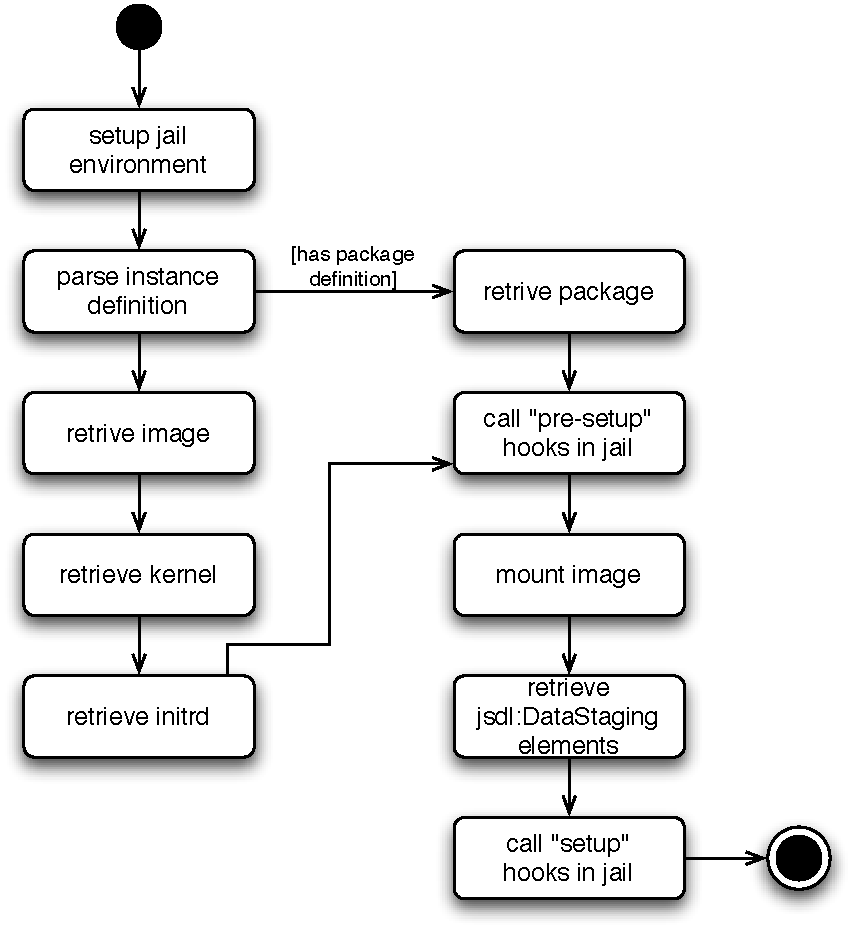
\includegraphics[scale=.55]{act-stage-in}
  \caption[Stage-In  Activity]{Overview  of  the  parts  of  the  stage-in
    activity.}
  \label{fig:act-stage-in}
\end{figure}

Now that all virtual machine specific files are available, the application
specific data can be retrieved. The \emph{xbed} assumes, that the image is
mountable by the UNIX \texttt{mount}  command and mounts it to a temporary
location within the jail environment.

All  JSDL-\texttt{DataStaging} elements that  define a  stage-in operation
are now handled with the  same retrieval mechanism as described above. The
paths that are used in the  job description are interpreted to be relative
to the mount point of the image.

Finally   the   ``setup''-hook  is   executed   using  the   user-supplied
scripts. These scripts  are given the path to  the image's mount-point and
can,  for  example,  decrypt  already  staged-in files  or  even  retrieve
additional input  data. If  everything went well,  the virtual  machine is
completely set up and can be started.

\subsubsection{Upload of files}

The upload of files from the execution environment to a location specified
by the user  is also accomplished by using  \gls{glo:URI}s. The process of
uploading a file is less  complicated than the retrieval process, since it
currently does  not involve compression or validation  directly.

The first step  after the virtual machine has been shut  down is again the
mounting of the image to a temporary location within the jail environment.
To provide  the possibility to  compress the files before  uploading them,
the ``cleanup'' hook is called before any of the actual staging operations
is called. The next step  is the handling of the JSDL-\texttt{DataStaging}
elements that  define a stage-out operation. The  only currently supported
protocols that can  be used for the upload  are \texttt{\gls{glo:FTP}} and
\texttt{\gls{glo:HTTP}}.  In the  final  step of  the  upload process  the
``post-cleanup''  hook is  called;  to that  time,  all specified  staging
operations have already been successfully performed and the image has been
unmounted.

If everything  went well, all  stored data\footnote{this does  not include
  internal data structures (\eg exit-code).}  that belongs to this task is
destroyed (\ie  the spool directory will  be deleted) and the  task is put
into the \texttt{Finished} state.

\subsection{Caching Of Arbitrary Files}
\label{sec:caching}

Compression   of  files   can   decrease  the   deployment  time   already
significantly, but  to avoid  long-distance transfers over  an unspecified
network connection, the  caching of files on the  server side is required,
this    follows    strictly    from    the    \emph{locality    principle}
\cite{locality-principle}.  The \emph{xbed} supports this by providing the
user with a  simple data-cache incorporated into the  system.  The user is
able to store  arbitrary data on the server prior submitting  a job to the
system. This makes the initialization  of a virtual machine for often used
images a lot faster compared  to always retrieving them over a potentially
slow network connection.

\subsubsection{Adding data to the cache}

An  user  adds  files  to   the  execution  environment  by  specifying  a
\gls{glo:URI} that can be retrieved by the \emph{xbed}.  This will usually
be the same \gls{glo:URI} the user would have given in his job description
(\eg a location  on some \texttt{\gls{glo:FTP}} or \texttt{\gls{glo:HTTP}}
server).  The \emph{xbed} attempts to retrieve the given \gls{glo:URI} and
adds a new entry to a database.

Actually the  complete mechanism  of caching is  implemented in  a special
component  within  the  \emph{xbed}  on   its  own.   The  cache  uses  an
\gls{glo:SQL}-database  to store information  about the  cached data  in a
persistent way. An user can add two different pieces of information to the
data he wants to have cached.  The first is the \textbf{type} of the data,
which can  be one  of \texttt{image}, \texttt{kernel},  \texttt{initrd} or
\texttt{data},  where the  \texttt{data} type  is just  a  placeholder for
arbitrary data  that does not fit  into one of the  other categories.  The
second piece of information is a \textbf{description}, that can be used to
describe the data in more detail,  \eg the version of a specific kernel, a
list of the applications that are installed within an image or the type of
compression   if  the   data   had  been   compressed.   Additionally   an
\texttt{SHA1}  digital fingerprint  of the  data is  computed  and stored,
along with the provided information, in the database.

The  cache-component  assigns each  entry  a  unique  identifier based  on
\gls{glo:UUID}s, this identifier  can later be used in  a \gls{glo:URI} to
refer to that  entry.  When using the \emph{xbe} command  line tool to add
data to  the cache, the \gls{glo:URI}  of the newly created  entry will be
printed on the screen upon success.

\subsubsection{Discovering cache entries}

The first way of ``discovering'' an  entry of the cache is simply to write
down the  \gls{glo:URI} one has received  upon addition of  the entry. But
that is not always feasible, since the entry could be shared among several
users who do not know each  other --- say, an administrator or provider of
a virtual machine image  added it to the cache, so that  it can be used by
several, to that time unknown, users.

The  discovery of  cached entries  is  implemented in  the \emph{xbed}  by
simply providing the  user with a list of all  entries. This list contains
most importantly the \gls{glo:URI} of the  entry, the type of data and the
description the submitter had given.

\begin{figure}[ht]
  \centering
  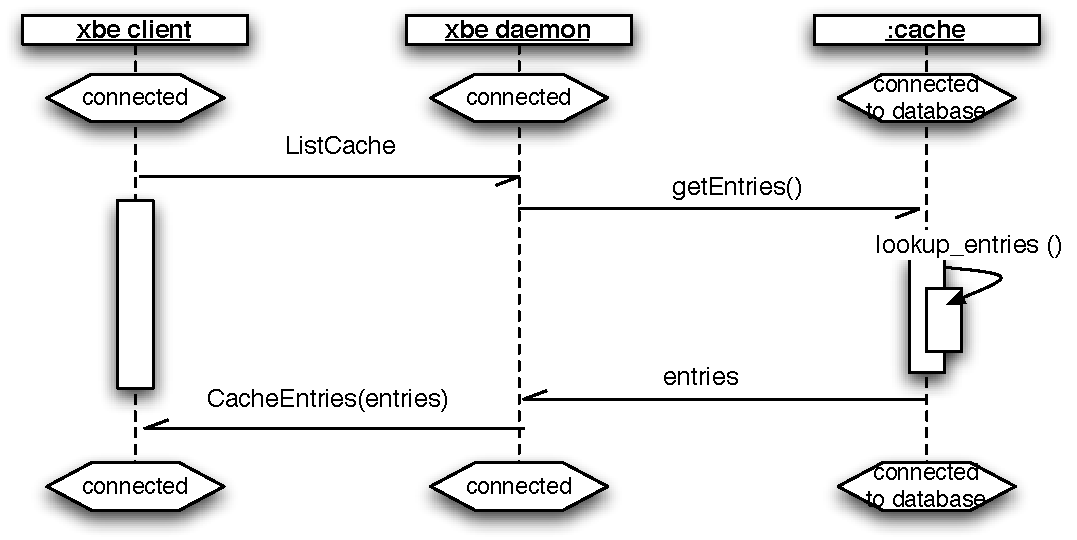
\includegraphics[scale=.55]{msc-list-cache}
  \caption[MSC List Cache Entries]{TODO: fill me in}
  \label{fig:msc-list-cache}
\end{figure}

The      \emph{Message     Sequence     Chart}      (\gls{glo:MSC})     in
Figure~\ref{fig:msc-list-cache} shows  the messages that  are sent between
the  client and  the server.   The client  requests a  list of  all cached
entries  by sending  the \texttt{ListCache}  message. Thereupon  makes the
\emph{xbed} a call to the cache-component  that provides him a list of all
entries. This list is eventually  transformed into an XML-message and sent
back to the client.  A sample output of the \texttt{xbe showcache} command
is shown in the following listing:

\bigskip

\begin{center}
  \begin{minipage}{.75\textwidth}
    \begin{lstlisting}[captionpos=b,backgroundcolor=\color{listingcolor},frame=lines,numbers=left,numberstyle=\tiny,caption={\emph{xbe} output of cache entries.},label={lst:xbe-listcache-out}]
<CacheEntries with 1 entry:
{'cache://xbe-file-cache/adfd0a99-4761-4816-8902-db8d62c8e482':
  {'description': 'Ubuntu kernel (2.6)',
   'hash': '732ca16f330c2c382e83cb997f5e027687a285aa',
   'type': 'kernel'}}
>
    \end{lstlisting}
  \end{minipage}
\end{center}

\subsubsection{Using cache entries}

Cache  entries can  be used  rather  easy. The  user is  just required  to
specify  the  \gls{glo:URI} of  a  cache  entry  instead of  the  original
\gls{glo:URI}.   The \emph{xbed} will  lookup the  specified \gls{glo:URI}
during the  stage-in process and  retrieve the data  from the cache,  if a
valid entry  could be found. The  same retrieval mechanism  applies to the
cached entries, so that compression  and validation can be used with them,
too.


\subsection[The Xen-based Submission Description Language]{The Xen-based Submission Description Language (XSDL)}
\label{sec:xen-based-submission}

This  section  describes  the   extensions  to  the  \emph{Job  Submission
  Description  Language} that  were developed.   The extensions  have been
required,  since   the  \gls{glo:JSDL}  does  not   directly  support  the
description of virtual machines.

There are actually two  different kinds of extensions: general extensions,
that  can also  be used  to enhance  some of  the  standard \gls{glo:JSDL}
elements, as well as an extension  that is purely specific to the proposed
execution environment.

\subsubsection{General extension elements}

As  described  above,  the  \gls{glo:XenBEE} supports  the  submission  of
compressed  files and  the  validation  of those  files  based on  digital
fingerprints.   To reflect this  behavior along  with the  job submission,
additional ``decorator''  elements have been  added.  Let me  clarify this
with  a  simple  example.   The  \gls{glo:JSDL} does  only  support  plain
\gls{glo:URI}s. If  this \gls{glo:URI} is now  used along with  one of the
decorators, the \emph{xbed} interprets the URI accordingly:

\bigskip

\begin{center}
  \begin{minipage}{.75\textwidth}
    \begin{lstlisting}[captionpos=b,backgroundcolor=\color{listingcolor},frame=lines,numbers=left,numberstyle=\tiny,caption={Example
        with the general \texttt{Hash} and \texttt{Compression}
        extensions.},label={lst:xbe-xsdl-example-hash},language=XML]
<jsdl:Source>
  <jsdl:URI>
    ftp://ftp.example.com/pub/input-file
  </jsdl:URI>
  <xsdl:Hash algorithm="sha1">
    a3b180e5dc2359849ffa927b93414ada20807a0c
  </xsdl:Hash>
  <xsdl:Compression algorithm="bzip2"/>
</jsdl:Source>
    \end{lstlisting}
  \end{minipage}
\end{center}

The    example   in   Listing~\ref{lst:xbe-xsdl-example-hash}\footnote{The
  namespace    prefixes    refer   to    the    namespaces   defined    in
  \emph{\nameref{sec:fundamentals:xml}},       Table~\ref{tab:namespaces}.}
could  be  an  excerpt  of  a  JSDL-\texttt{DataStaging}  operation.   The
\texttt{Source} element contains the URI that refers to the location of an
input file which shall be staged in.

The \texttt{Hash}  extension stores the digital fingerprint  of the source
file and the algorithm that has been used to generate it. This fingerprint
is used by  the \emph{xbed} to verify that the  retrieved file is actually
the same  as on the  server. The \texttt{Compression} extension  holds the
algorithm only --- one  of \texttt{bzip2}, \texttt{gzip}, \texttt{tbz} and
\texttt{tgz} ---  that has been used  to compress the file.  In this case,
the  file  \texttt{input-file}   is  compressed  with  the  \texttt{bzip2}
algorithm.

An XML-Schema document is used to validate each one of the extensions. For
example,  the  compression  algorithm  is  checked  against  the  list  of
supported  algorithms and  the  content of  the  \texttt{Hash} element  is
restricted to hexadecimal digits.

\medskip

When the document is parsed a  special class will be instantiated for each
of    these   elements.    That    are   the    \texttt{Compression}   and
\texttt{HashValue} classes. Both are initialized with the parameters given
to the element  and are used to decompress or  validate the retrieved file
respectively.

\subsubsection{\gls{glo:XenBEE} specific extensions}

The staging operations  that are provided by the  \gls{glo:JSDL} cannot be
used  to  describe   the  required  files  for  a   virtual  machine  (\ie
\emph{image}, \emph{kernel} and  \emph{initrd}). Those operations ``work''
on the file-system hierarchy that  is perceived by the application itself,
and that is already the file-system of the virtual machine.

However, the virtual machine specific files  have to be staged in as well,
so there  was a need  to provide an  extension to the  \gls{glo:JSDL}. The
extension follows  the \gls{glo:JSDL} in the  way it is  structured and is
added as an additional element to the JSDL-\texttt{Resources} element. The
extension  defines an  \texttt{InstanceDefinition} element  which contains
the  actual \texttt{InstanceDescription}.  The  following listing  shows a
thorough example usage of this extension.

\bigskip

\begin{center}
  \begin{minipage}{.75\textwidth}
    \begin{lstlisting}[captionpos=b,backgroundcolor=\color{listingcolor},frame=lines,numbers=left,stepnumber=5,numberfirstline=false,numberstyle=\tiny,caption={Example
      of an \texttt{InstanceDefinition} element describing the required
      files of a virtual machine.},label={lst:xbe-xsdl-example},language=XML]
<xsdl:InstanceDefinition>
  <xsdl:InstanceDescription>
    <xsdl:Instance>
      <xsdl:Image fs-type="ext3">
        <xsdl:Location>
          <xsdl:URI>
            http://www.example.com/base.img
          </xsdl:URI>
        </xsdl:Location>
      </xsdl:Image>
      <xsdl:Kernel>
        <xsdl:Location>
          <xsdl:URI>
            http://www.example.com/kernel
          </xsdl:URI>
        </xsdl:Location>
      </xsdl:Kernel>
      <!-- the initrd is optional -->
      <xsdl:Initrd>
        <xsdl:Location>
          <xsdl:URI>
            http://www.example.com/initrd
          </xsdl:URI>
        </xsdl:Location>
      </xsdl:Initrd>
    </xsdl:Instance>
  </xsdl:InstanceDescription>
</xsdl:InstanceDefinition>
    \end{lstlisting}
  \end{minipage}
\end{center}

Each one of the special files has its own element, \ie the \texttt{Image},
\texttt{Kernel} and  \texttt{Initrd} element, whereas  the \texttt{Initrd}
element is optional. The locations of the files are specified by using the
\texttt{Location}  element  that  contains  a  \gls{glo:URI}.   The  image
specification can  contain an additional  attribute that defines  the used
file-system  ---  currently   only  \texttt{ext2}  and  \texttt{ext3}  are
supported\footnote{Both of  them are standard file-systems  found on Linux
  systems.}.   The generic extensions  discussed before  can be  used with
\texttt{Location} elements as well.

The here defined  files are staged directly into  the spool directory that
has   been  created  exclusively   for  this   single  job,   whereas  the
JSDL-\texttt{DataStaging} files are retrieved into the image.

\section[The Xen-Based Execution Instance Daemon]{The Xen-Based Execution Instance Daemon (xbeinstd)}
\label{sec:xbeinstd}

The  \emph{Xen-Based  Execution  Instance   Daemon}  is  a  rather  simple
component   which  runs   within  a   virtual  machine   created   by  the
\emph{xbed}. The user  or the person who provides the  image for a virtual
machine  is  required  to  install  this daemon  inside  the  image  prior
submission. The daemon  must also be started during  the initialization of
the operating system (an \texttt{init}-script to start and stop the daemon
on UNIX-like systems is provided in the source package).

When the \emph{xbed} creates a  new virtual machine it adds two parameters
to the kernel which are eventually exported to the \texttt{init}-script as
environment variables.  The first parameter contains the unique identifier
of the instance,  so that a two-way communication  based on message-queues
can  be established,  whereas  the second  contains  a \gls{glo:URI}.  The
\gls{glo:URI}\footnote{The   URI   could,    for   example,   look   like:
  \url{stomp://mqs.example.com/xenbee.daemon.1}}       specifies       the
message-queue  server and  the queue  that shall  be used  to  contact the
\emph{xbed}.

\subsubsection{Startup of the xbeinstd}

On  startup,  the \emph{xbeinstd}  uses  the  \gls{glo:URI}  given in  the
environment variable  \texttt{XBE\_SERVER} or as a  command line parameter
to  connect  to  the  message-queue  server.  When  the  connection  could
successfully be  established, the  \emph{xbeinstd} subscribes itself  to a
unique  queue which  uses  the identifier  of  the virtual  machine it  is
running on.

Now that  the \emph{xbeinstd}  is completely set  up, it  notifies ``his''
\emph{xbed}  that  it  is  available  now. Therefore  it  sends  a  simple
\texttt{InstanceAvailable} message to the  \emph{xbed} and waits for a job
that   it  can   execute.   Additionally   to  that,   it   sends  regular
\texttt{InstanceAlive} message to the \emph{xbed}. These messages tell the
\emph{xbed} that the instance is still functional\footnote{The \emph{xbed}
  shuts virtual  machines down,  if they do  not send  keep-alive messages
  regularly.},  they also contain  some informational  values such  as the
uptime and idle-time of the virtual machine.

\subsubsection{Execution of the user's application}

Once the \emph{xbed}  is aware of the availability  of the virtual machine
and  the   \emph{xbeinstd},  it  sends  the  job   description  using  the
\texttt{ExecuteTask} message to  the virtual machine. The \emph{xbeinstd},
in turn, parses the \gls{glo:JSDL} document contained in this message.

The    JSDL     supports    the    description     of    executables    on
\gls{glo:POSIX}-compliant  systems  using the  \texttt{POSIX\-Application}
extension. The individual  steps that lead eventually to  the execution of
the application can be summarized as follows:

\begin{itemize}
\item The  \texttt{Executable}, \texttt{Argument} and \texttt{Environment}
  elements are parsed.  These values are assembled to  the parameters that
  are eventually passed to the \texttt{execve} system-call.
\item  The  input,  output  and  error  streams  of  the  application  are
  redirected  either to the  files specified  in the  JSDL document,  or to
  \texttt{/dev/null}.
\item  The working  directory  of the  application  is set  either to  the
  directory specified in the JSDL document, or to \texttt{``/''}.
\item  Finally the  application  is executed  as  a child  process of  the
  \emph{xbeinstd}.
\end{itemize}

Additionally   to  the   environment  variables   specified  in   the  job
description, the  \texttt{MQS} environment variable is  set.  Per default,
this  variable is  set to  the message-queue  server that  is used  by the
\emph{xbeinstd},  but the  value can  be overridden  by an  user  using an
\texttt{Environment} element  that defines this  variable.  An application
that is  distributed over  several virtual machines  can make use  of this
variable for communication and coordination purposes.

When the application finishes  its execution, the \emph{xbeinstd} notifies
the   \emph{xbed}   about   that   using   an   \texttt{ExecutionFinished}
message. The  daemon does  not terminate itself,  it rather waits  for the
\emph{xbed} to shut the virtual machine down. I decided to implement it in
that way, to have the option to possibly reuse the virtual machine, \ie in
the future, it  could be possible to execute more  than one application in
the same virtual machine.

\subsubsection{On-demand virtual machine deployment}

In the  previous section  I have described  how ordinary  applications are
executed  with  the  \emph{xbeinstd},  but  those  applications  typically
terminate after some  time. The on-demand deployment of  a virtual machine
does not aim at the execution  of an application specified in the JSDL, it
just aims at the creation of the virtual machine.

To keep the  \emph{xbeinstd} simple, the best way was  to define a special
extension to  the JSDL.  This  extension aims at  the \texttt{Application}
element   just  as   the  POSIX   extensions.   The   element   is  called
\texttt{XBEApplication}.  The  following listing  shows the usage  of this
extension.  The  only ``executable''  that  is  currently  defined is  the
\texttt{ContinuousTask}.

\bigskip

\begin{center}
  \begin{minipage}{.75\textwidth}
    \begin{lstlisting}[captionpos=b,backgroundcolor=\color{listingcolor},frame=lines,numbers=none,stepnumber=5,numberfirstline=false,numberstyle=\tiny,caption={Example
        of a \texttt{ContinuousTask} used for on-demand virtual machine deployment.},label={lst:xbe-xbeinstd-continuous-task},language=XML]
<jsdl:Application>
  <xbe:XBEApplication>
    <xbe:ContinuousTask/>
  </xbe:XBEApplication>
</jsdl:Application>
    \end{lstlisting}
  \end{minipage}
\end{center}

When  the \emph{xbeinstd}  encounters  this specific  \texttt{Application}
element, it does  nothing, actually.  The user must log  in to the created
virtual machine, \eg by using a remote shell such as \gls{glo:SSH}.

\section[The Xen-Based Execution Command Line Client]{The Xen-Based Execution
  Command Line Client (xbe)}
\label{sec:command-line-client}

The implemented  command line  client is very  straightforward to  use. It
provides the user with an  on-line help system, which provides information
about all supported commands and how they are used. The help system can be
activated by issuing the \texttt{xbe help} shell command in a terminal.

The  \emph{xbe}  has  an  interface   to  all  aspects  of  the  execution
environment  that  have been  discussed  so far.   It  allows  an user  to
\texttt{reserve}, \texttt{confirm} or \texttt{terminate} a reservation and
it  is   also  possible  to   monitor  the  \texttt{status}  of   a  given
reservation. The tool too has an interface to the cache and it is able add
data to  the cache  and list  the current contents  by using  the commands
\texttt{cache} and \texttt{showcache}, respectively.

Since the protocol assumes a two-step  process for the submission of a new
job  (\ie creation  and  confirmation of  a  reservation), the  \emph{xbe}
provides a  convenience command,  that allows an  user to perform  the two
steps in one  \texttt{submit} command. The \texttt{submit} as  well as the
\texttt{confirm} commands  require the job definition  as a \gls{glo:JSDL}
document.   The  creation   of  such  a  document  is   not  part  of  the
\gls{glo:XenBEE},  but several example  files are  included in  the source
distribution.

\medskip

The  next  section  is  going  to discuss  the  implemented  message-based
communication protocol in detail.

\section{The Communication Protocol Stack}
\label{sec:communication-protocol}

The three components,  that have been discussed in  the previous sections,
are  using  message-queues  and  one  or  more  message-queue  servers  to
communicate with each other.

This section  describes the details of the  communication architecture and
its  individual  layers.  There  are  four  layers, the  \emph{Application
  Layer},  that  implements  the  behavior  of each  single  message,  the
\emph{XML Message Layer} that represents  each message as an XML document,
the  \emph{Security  Layer} which  provides  authenticity  and privacy  as
described            in            Section~\ref{sec:secure-communication},
\emph{\nameref{sec:secure-communication}},  and at  the  lowest level  the
\emph{STOMP  Layer} which  is  used to  communicate  with a  message-queue
server.  An overview over  the layers  in shown  in the  following diagram
(Figure~\ref{fig:communication-layers}).

\medskip

\begin{figure}[ht]
  \centering
  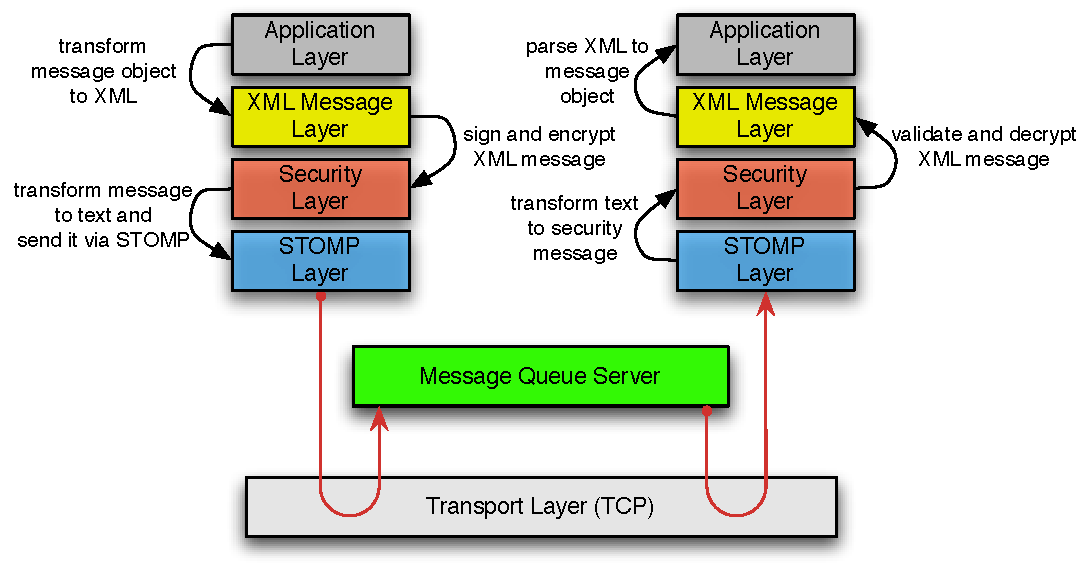
\includegraphics[scale=.7]{protocol-layers}
  \caption[Protocol  Layers]{The  individual   protocol  layers  that  are
    involved when sending a message to another component.}
  \label{fig:communication-layers}
\end{figure}

In the \emph{Application Layer} a  message is represented by an object, so
that information contained in the  message can easily be read and written.
The message  is then  transformed into an  XML-document and passed  to the
next layer, \ie the \emph{XML Message Layer}. The \emph{Security Layer} is
actually  an XML-based  layer,  too,  it signs  and  encrypts the  message
received from  the upper layer in  an XML-message.  The final  step is the
sending of the message  to the communication partner's message-queue using
the STOMP protocol.

\medskip

The following sections describe the common format of the XML messages that
are used in the security layer as well as in the message layer. After that
each layer of the protocol stack is discussed in detail, starting with the
STOMP layer.  The application  layer is not  described here, since  it has
already been covered in the previous sections.

\subsection{XML Messages}

The  XML messages  that  are used  in  the \emph{Security  Layer} and  the
\emph{XML Message Layer} share a  common structure. The messages are split
into two parts \emph{MessageHeader}  and \emph{MessageBody} which are both
children of the top-level \emph{Message} element.

The  header,  for  example,  may  contain  security  related  information,
currently it is  only used by the security layer.   The body, however, can
either be empty, too, or  contain another XML document that represents the
application data.

\medskip
\begin{center}
  \begin{minipage}{.75\textwidth}
    \begin{lstlisting}[captionpos=b,backgroundcolor=\color{listingcolor},frame=lines,numbers=none,stepnumber=5,numberfirstline=false,numberstyle=\tiny,caption={The
        structure of an XML message.},label={lst:xml-message-example},language=XML]
<xbe:Message>
   <xbe:MessageHeader>
     <!-- security related information -->
   </xbe:MessageHeader>
   <xbe:MessageBody>
     <!-- payload XML document representing
          application data. For example:
          an encrypted XML document -->
   </xbe:MessageBody>
</xbe:Message>
    \end{lstlisting}
  \end{minipage}
\end{center}

To transfer an XML document, the internal tree representation is converted
into a textual  representation and then sent to  the communication partner
through the lower transportation layer.

\subsection{The STOMP Layer}
\label{sec:protocol:stomp}

The  \emph{Streaming  Text  Oriented Message  Protocol}  (\gls{glo:STOMP})
\cite{stomp} is the  layer at the lowest level and  is used to communicate
with  a  message-queue  server.

When  one  of  \gls{glo:XenBEE}'s  components wants  to  communicate  with
another   component,  it   connects  to   a  message-queue   server  using
\gls{glo:TCP}.    This   connection   can   now  used   to   establish   a
Stomp-connection. If  an user wants  to request the  status of one  of his
submissions,  he  passes an  \gls{glo:URI}  to  the  \emph{xbe}. This  URI
contains   the  low-level   transport  mechanism,   the  address   of  the
message-queue server and  the queue that must be  used to communicate with
the other side.  Consider the following URI:
\begin{quote}
  \url{stomp://mqs.example.com:61613/a}
\end{quote}
It specifies,  that Stomp should be  used to connect  to the message-queue
server that is listening at the given address. To reach the service on the
other  side,  messages  are  sent  to the  queue  \texttt{``a''}  on  this
message-queue server.

Since the available Stomp clients  for Python did not meet my expectations
and requirements --- they did not integrate well with the \texttt{twisted}
framework,  I  implemented  the   client  side  of  the  protocol  myself.
Therefore, the source distribution  of \gls{glo:XenBEE} includes a generic
implementation of the  Stomp protocol that can be  used in other projects,
as well.  Additionally, a  small command line  tool (\texttt{stompclient})
has  been  implemented, that  can  be used  for  testing  purposes ---  it
supports  the  subscription to  multiple  message-queues  as  well as  the
transmission of files to an arbitrary destination queue.

\subsection*{Protocol Description}

The Stomp protocol comes ``from the HTTP school of design'' and the client
is really easy to implement. The  site at \cite{stomp} states, that even a
\texttt{telnet} session can be used to communicate with a Stomp server.

The  messages  that  are  sent   between  client  and  server  are  called
\emph{Frames}  and consist of  three parts:  \emph{Command}, \emph{Header}
and \emph{Body}.   The \emph{Command} defines  the type of the  frame (\eg
\texttt{SUBSCRIBE} is used to subscribe  to a message-queue on the server,
\texttt{SEND} is  used to send an application  message). The \emph{Header}
consists of key-value pair lines; the  header's end is denoted by an empty
line. The \emph{Body} contains the payload  of the frame and is ended by a
\texttt{null} (control-@  in ASCII) byte. This section  does only describe
those   frames  that   are   relevant  to   the   implementation  of   the
\gls{glo:XenBEE}.

\subsubsection{Connecting to a Stomp Server}

After  a  client   is  connected  to  a  Stomp-server,   \eg  by  using  a
TCP-connection, it has to login  before it can actually use the connection
to  send  and  receive  messages   ---  this  is  achieved  by  sending  a
\texttt{CONNECT} frame to the server as shown in the following listing:

\medskip
\begin{center}
  \begin{minipage}{.75\textwidth}
    \begin{lstlisting}[captionpos=b,backgroundcolor=\color{listingcolor},frame=lines,numbers=none,stepnumber=5,numberfirstline=false,numberstyle=\tiny,caption={The initial
      \texttt{CONNECT} message sent by a Stomp client.},label={lst:stomp-connect}]
CONNECT
login: <username>
passcode: <passcode>

^@
    \end{lstlisting}
  \end{minipage}
\end{center}

The \texttt{CONNECT} frame supports two header elements, \texttt{username}
and  \texttt{passcode} that  can be  used by  the server  administrator to
restrict  the   access  to  the   server.  The  server  sends   either  an
\texttt{ERROR}  frame  which   contains  detailed  information  about  the
occurred error or it sends the \texttt{CONNECTED} frame:

\medskip
\begin{center}
  \begin{minipage}{.75\textwidth}
    \begin{lstlisting}[captionpos=b,backgroundcolor=\color{listingcolor},frame=lines,numbers=none,stepnumber=5,numberfirstline=false,numberstyle=\tiny,caption={The
        \texttt{CONNECTED} message sent by a Stomp server after a client
        has successfully logged in.},label={lst:stomp-connected}]
CONNECTED
session-id: <session-id>

^@
    \end{lstlisting}
  \end{minipage}
\end{center}

According to  the Stomp protocol specification found  in \cite{stomp}, the
\texttt{session-id}  header  element  is  a  unique  identifier  for  this
session, but it is not actually used yet.

\subsubsection{Subscribing to Message-Queues}

A Stomp client may subscribe to as  many queues or topics as it likes. The
Stomp server takes control of  the subscriptions and forwards all messages
that  are targeted  at  a  particular queue  or  topic. \emph{Topics}  and
\emph{queues} differ mainly  in the way messages are  handled. A topic has
the semantics  of a $m:n$ communication, \ie  a message that is  sent to a
topic will be received  by \textbf{all} subscribers. \emph{Queues}, on the
other hand,  have $m:1$ semantics ---  a sent message is  only received by
\textbf{at most one} client that is subscribed to that queue. If more than
one client did subscribe to the same queue, the server may randomly select
one of them to be the receiver.

\medskip
\begin{center}
  \begin{minipage}{.75\textwidth}
    \begin{lstlisting}[captionpos=b,backgroundcolor=\color{listingcolor},frame=lines,numbers=none,stepnumber=5,numberfirstline=false,numberstyle=\tiny,caption={The
        \texttt{SUBSCRIBE} frame used for queue or topic subscription.},label={lst:stomp-subscribe}]
SUBSCRIBE
destination: /queue/foobar
ack: client

^@
    \end{lstlisting}
  \end{minipage}
\end{center}

The  frame  that  is  shown  above  subscribes the  client  to  the  queue
\texttt{foobar} and  will receive messages  targeted to that  queue. Stomp
distinguishes   queues   and   topics   by   special   prefixes   in   the
\texttt{destination}    header    element,    \ie   \texttt{/queue}    and
\texttt{/topic}, respectively. The header element \texttt{ack} can take on
two different  values \texttt{client} and  \texttt{auto}. If it is  set to
\texttt{client}, the  recipient of the  message must send  an \texttt{ACK}
frame to acknowledge the reception,  otherwise the frame is not considered
to  be  delivered  and  will  be  sent  again later.   If  it  is  set  to
\texttt{auto}, the  frame will be sent  only once\footnote{A message-queue
  server delivers messages not until  at least one client is subscribed to
  that queue.}  and is discarded afterwards.

The  components of  the  \gls{glo:XenBEE} use  queues  to establish  their
communication.   The \emph{xbed}  subscribes to  a queue  that  looks like
\texttt{xenbee.daemon.<unique-id>},  however, the actual  queue has  to be
configured by  an administrator  (\ie specify the  unique identification).
The    \emph{xbeinstd}    subscribes     to    queues    of    the    form
\texttt{xenbee.instance.<UUID>} ---  the UUID is the  unique identifier of
the virtual machine  instance. The \emph{xbe} is no  exception to that and
subscribes to queues of  the form \texttt{xenbee.client.<UUID>}, where the
UUID is randomly chosen.

To  end   a  previously  made   subscription,  the  client  can   send  an
\texttt{UNSUBSCRIBE} frame. The following listing cancels the subscription
to the \texttt{foobar} queue:

\medskip
\begin{center}
  \begin{minipage}{.75\textwidth}
    \begin{lstlisting}[captionpos=b,backgroundcolor=\color{listingcolor},frame=lines,numbers=none,stepnumber=5,numberfirstline=false,numberstyle=\tiny,caption={The
        \texttt{UNSUBSCRIBE} frame revokes a previously made subscription.},label={lst:stomp-unsubscribe}]
UNSUBSCRIBE
destination: /queue/foobar

^@
    \end{lstlisting}
  \end{minipage}
\end{center}


\subsubsection{Sending and Receiving Messages}

To  send   application  data  to   another  entity,  the  sender   uses  a
\texttt{SEND}  frame.    An  example   of  such  a   frame  is   shown  in
Listing~\ref{lst:stomp-send}. The shown  frame represents the transmission
of the  message ``Hello  World!'' (without the  quotation marks)  to queue
\texttt{a}.  The \texttt{reply-to} header  is used  to tell  the receiving
entity to which queue it has to address its replies.

\medskip
\begin{center}
  \begin{minipage}{.75\textwidth}
    \begin{lstlisting}[captionpos=b,backgroundcolor=\color{listingcolor},frame=lines,numbers=none,stepnumber=5,numberfirstline=false,numberstyle=\tiny,caption={The
        \texttt{SEND} frame is used to send application data.},label={lst:stomp-send}]
SEND
destination: /queue/a
reply-to: /queue/b
content-length: 12

Hello World!^@
    \end{lstlisting}
  \end{minipage}
\end{center}

The  \texttt{content-length}  header  defines  the actual  length  of  the
payload  (the empty  line between  header and  body marks  the end  of the
header).   The   string  ``Hello   World!''   consists  of   exactly  $12$
characters.  The Stomp client can  now be sure that the next \texttt{null}
byte indeed marks the end of this frame.  If no \texttt{content-length} is
specified,  the Stomp  client assumes  that the  frame ends  at  the first
occurrence of a  \texttt{null} byte.  Depending on the  payload data, this
can be  harmful ---  consider, for example,  the transmission of  raw, \ie
non-ASCII, data, in this type of  data a \texttt{null} byte is very likely
to occur.

This message is transmitted by the server to one of the consumers that are
subscribed to  the queue \texttt{``a''}.  The following listing  shows how
the resulting frame could probably look like:

\medskip
\begin{center}
  \begin{minipage}{.75\textwidth}
    \begin{lstlisting}[captionpos=b,backgroundcolor=\color{listingcolor},frame=lines,numbers=none,stepnumber=5,numberfirstline=false,numberstyle=\tiny,caption={The
        \texttt{MESSAGE} frame is used by the server to transmit a message
        to a client.},label={lst:stomp-message}]
MESSAGE
destination: /queue/a
message-id: <message-identifier>
reply-to: /queue/b
content-length: 12

Hello World!^@
    \end{lstlisting}
  \end{minipage}
\end{center}

The   header    elements   \texttt{destination},   \texttt{reply-to}   and
\texttt{content-length} are still  the same. But a new  header element has
been added  by the server,  too.  The \texttt{message-id}  header uniquely
identifies  this  message  ---   if  the  queue-subscription  was  set  to
\texttt{client}-acknowledge mode,  this identifier has  to be used  in the
subsequent \texttt{ACK} frame.

\medskip

This  concludes  the  basic  transportation  layer that  is  used  in  the
\gls{glo:XenBEE}. All  messages that are  received by the Stomp  layer are
forwarded to the upper layer and will be handled by specialized protocols.

\subsection{The Security Layer}
\label{sec:protocol:security}

This layer  implements the \emph{Message Layer  Security} functionality as
described in Section~\ref{sec:fundamentals:mls}.  The protocol is based on
XML  messages that  are  sent  through the  lower  layer.  Currently,  the
\emph{Security Layer} is only used in the communication between \emph{xbe}
and \emph{xbed}, \ie between user and server.

The protocol is split into  two phases, an \emph{initialization phase} and
the actual \emph{communication phase}. During the initialization phase the
communication partners  exchange their public-key certificates  and set up
the  encryption  scheme  that  shall  be  used in  the  next  phase.   The
certificates are then validated  against a Certificate Authority to verify
the identity  of the  communication partner. The  subsequent communication
phase uses  the exchanged  information of the  first phase  and transports
application data in a secure way (\ie digitally signed and encrypted).

\subsubsection{Initialization Phase}

This phase is  entered whenever one of the endpoints wants  to start a new
communication with another endpoint. That means both sides can establish a
new connection, but most  of the time it will be the  client side (\eg the
\emph{xbe}) that initiates the connection. Before the actual communication
can  be secured,  the public-key  certificates of  both endpoints  must be
exchanged.

\begin{figure}[ht]
  \centering
  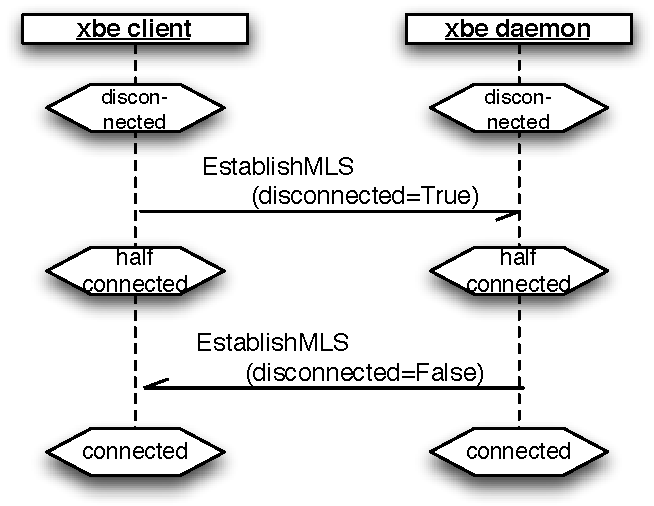
\includegraphics[scale=.55]{msc-establish-mls}
  \caption[MSC    Message   Layer    Security]{Exchange    of   public-key
    certificates.}
  \label{fig:msc-establish-mls}
\end{figure}

The   \gls{glo:MSC}  in  Figure~\ref{fig:msc-establish-mls}   shows  which
messages are sent to establish  a secure communication. They start both in
the \texttt{disconnected}  state and the client  starts the initialization
process  by sending a  \texttt{EstablishMLS} message  to the  server. This
message contains the client's certificate  and the signature in the header
of the message.  The message also says that the client is currently in the
\texttt{disconnected} state which tells the server to send his certificate
as well.

The  server  receives  the  message,  verifies  its  signature  using  the
certificate included in the message and finally validates this certificate
against a  \gls{glo:CA}. If  the certificate is  valid, the  server checks
whether the  certificate owner  is authorized to  connect at all.   If the
certificate could not be validated (\ie the signature did not match or the
certificate  was not  issued  by the  \gls{glo:CA})  or the  owner of  the
certificate is disallowed to connect, an \texttt{Error} message indicating
the reason for failure is sent back. If the user is allowed to connect and
the   received   message   has    been   valid,   the   server   sends   a
\texttt{EstablishMLS},  too.  As  requested  by the  client, this  message
includes the server's certificate, but this time the \texttt{disconnected}
flag is set to \texttt{false}.

All transmitted messages are digitally signed by the sender. At the end of
the two-way handshake, both sides  know the other's certificate, so that a
public-key based, secure communication can be established.

\subsubsection{Communication Phase}

This phase  handles the signing  and encryption of the  actual application
data  (\emph{payload messages}).  The  signature of  the payload  is added
directly  to   the  \texttt{MessageHeader}  of  the   payload,  while  the
encryption  of  a  message  creates  a  new  message,  the  \emph{envelope
  message}.   The schematic  process of  transmitting a  message  from the
\emph{xbe} to the \emph{xbed} is shown in Figure~\ref{fig:net-mls}.
 
\begin{figure}[ht]
  \centering
  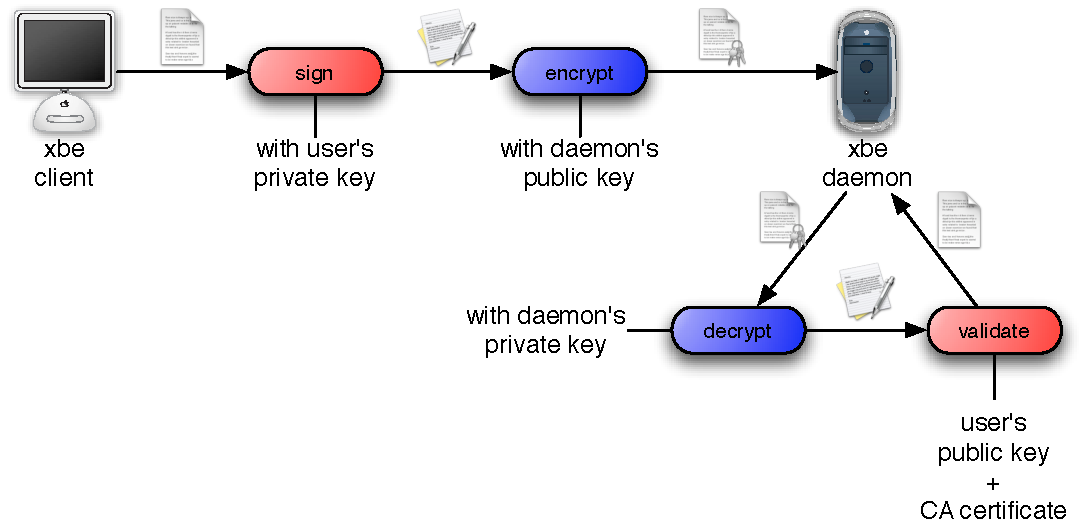
\includegraphics[scale=.55]{message-layer-security}
  \caption[Message Layer Security]{Secure transmission of an XML document.}
  \label{fig:net-mls}
\end{figure}

Before a message  is encrypted, it is signed by  the sender, the procedure
for generating the signature can be summarized in the following steps:

\begin{itemize}
\item     Generate     the     canonical     representation     of     the
  \emph{payload-message's} XML document (see \cite{canonical-xml} for more
  information on \emph{Canonical XML}).
\item  Transform this  canonical form  into a  textual  representation and
  compute its digital fingerprint using a secure hash algorithm.
\item Sign this digital fingerprint  with the sender's private key and add
  the resulting signature to the header of the payload message.
\end{itemize}

To validate such  a message, the recipient must  remove the signature from
the message's header first. Now  he can compute the digital fingerprint of
the message in the same way  as the sender.  Finally, to actually validate
the message, the  signature is validated with the  sender's public-key ---
if the result is equal to the fingerprint, the message is valid.

The next step is the encryption  of the signed message, therefore the just
mentioned  envelope message is  created.  The  encryption is  performed by
using  a   symmetric  encryption  algorithm  with   a  randomly  generated
key\footnote{The  current  implementation  uses the  \texttt{DES-EDE3-CBC}
  algorithm.  Detailed information  on this algorithm can be  found in RFC
  $2420$, \emph{The  PPP Triple-DES  Encryption Protocol}.}.  This  key is
then itself  encrypted using the  recipient's public-key and added  to the
header of the envelope message.  The  body of the envelope consists of the
\texttt{\gls{glo:base64}}   encoded,  encrypted  original   message.   The
skeleton    of     such    an    envelope    message     is    shown    in
Listing~\ref{lst:encrypted-message-skeleton}.

\medskip
\begin{center}
  \begin{minipage}{.75\textwidth}
    \begin{lstlisting}[captionpos=b,backgroundcolor=\color{listingcolor},frame=lines,numbers=none,stepnumber=5,numberfirstline=false,numberstyle=\tiny,caption={The
        skeleton of an encrypted message.},label={lst:encrypted-message-skeleton},language=XML]
<xbe:Message>
  <xbe:MessageHeader>
    <xbe-sec:CipherInfo>
      <xbe-sec:CipherKey>
        <!-- base64 encoded encrypted key -->
      </xbe-sec:CipherKey>
      <xbe-sec:CipherIV>
        <!-- base64 encoded Initialization Vector -->
      </xbe-sec:CipherIV>
      <xbe-sec:CipherAlgorithm>
        <!-- the algorithm used to encrypt/decrypt the data -->
      </xbe-sec:CipherAlgorithm>
    </xbe-sec:CipherInfo>
  </xbe:MessageHeader>
  <xbe:MessageBody>
    <xbe-sec:CipherData>
      <xbe-sec:CipherValue>
        <!-- base64 encoded encrypted message -->
      </xbe-sec:CipherValue>
    </xbe-sec:CipherData>
  </xbe:MessageBody>
</xbe:Message>
    \end{lstlisting}
  \end{minipage}
\end{center}


\subsubsection{Implementation Details}


\begin{itemize}
\item symmetric encryption one-time key
\item signing of whole message
\item encryption of body
\item xml-message-security
\end{itemize}
\subsubsection{m2crypto / openssl}

\begin{itemize}
\item problems with m2crypto on 64bit architecture
\item both are currently incompatible to each other
\item both sides (client/server) have to use the same --- either m2 or
  direct openssl
\end{itemize}


\subsection{MSCs}

\begin{itemize}
\item make reservation
\item confirm reservation (jsdl) +/- start
\item submit whole job (make res + confirm)
\item terminate activity
\item status request
\item add cache entry
\item security establishment (certificates, encryption, signing)
\item stomp
\end{itemize}


\begin{figure}[ht]
  \centering
  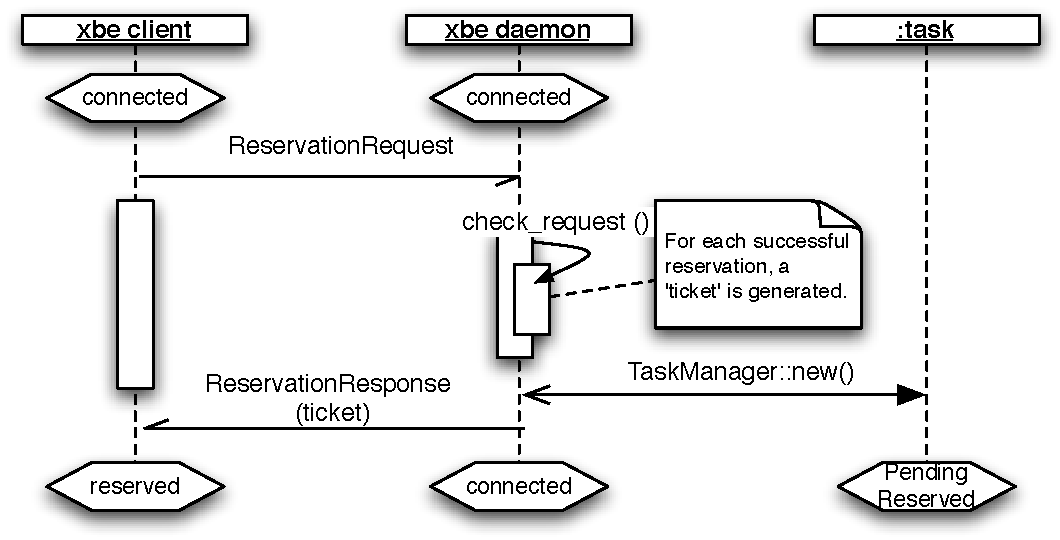
\includegraphics[scale=.75]{msc-reserve}
  \caption[MSC Make Reservation]{TODO: fill me in}
  \label{fig:msc-reserve}
\end{figure}

\begin{figure}[ht]
  \centering
  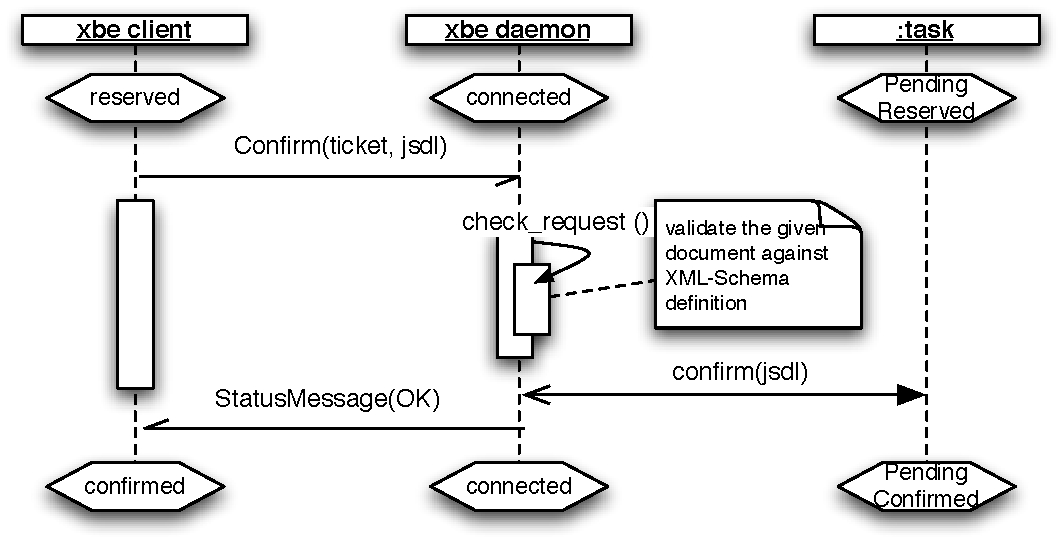
\includegraphics[scale=.75]{msc-confirm}
  \caption[MSC Confirm Reservation]{TODO: fill me in}
  \label{fig:msc-confirm}
\end{figure}

\begin{figure}[ht]
  \centering
  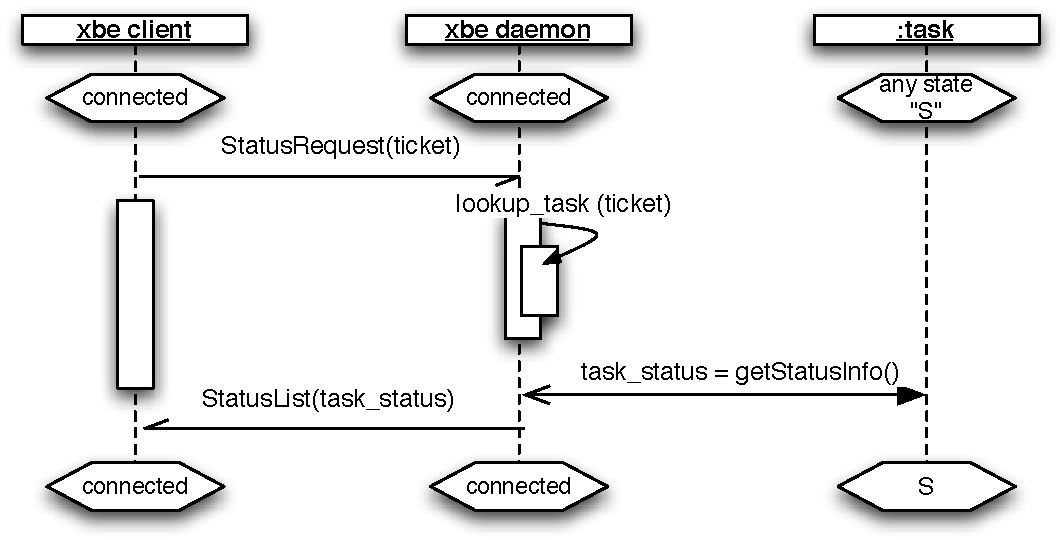
\includegraphics[scale=.75]{msc-status-request}
  \caption[MSC Request Task Status]{TODO: fill me in}
  \label{fig:msc-status-request}
\end{figure}

\begin{figure}[ht]
  \centering
  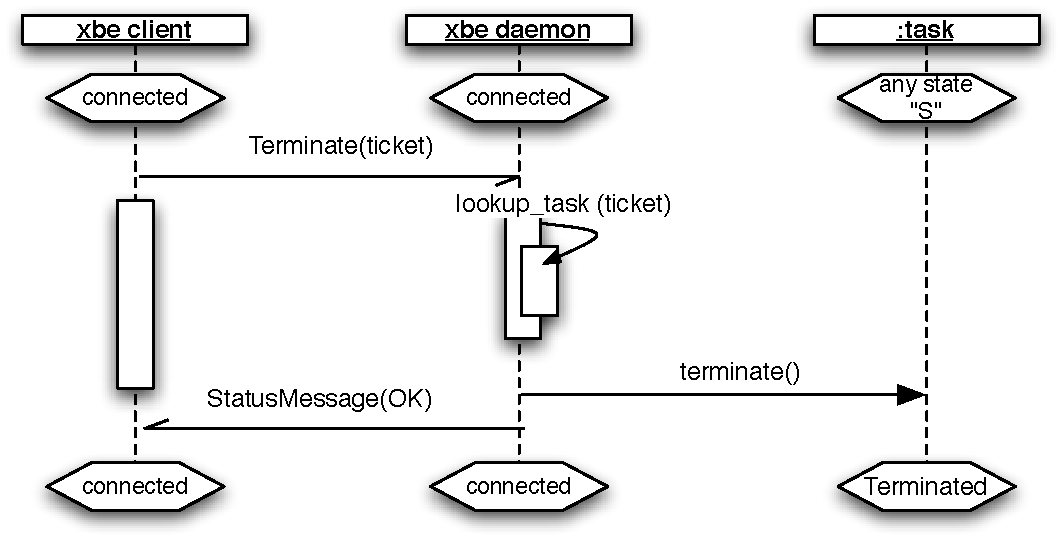
\includegraphics[scale=.75]{msc-terminate}
  \caption[MSC Terminate Task Request]{TODO: fill me in}
  \label{fig:msc-terminate}
\end{figure}

\subsection{Network Topology}
\label{sec:network-topology}

\begin{itemize}
\item simple topology: just one mqs (preferably on the xbed-host)
\item advanced topology: many mqs with configured forwarding
\item avoids common problems that arise with NAT and firewall policies
\item xbeinstd and possibly the application use the same mqs as the xbed
\end{itemize}

\begin{figure}[ht]
  \centering
  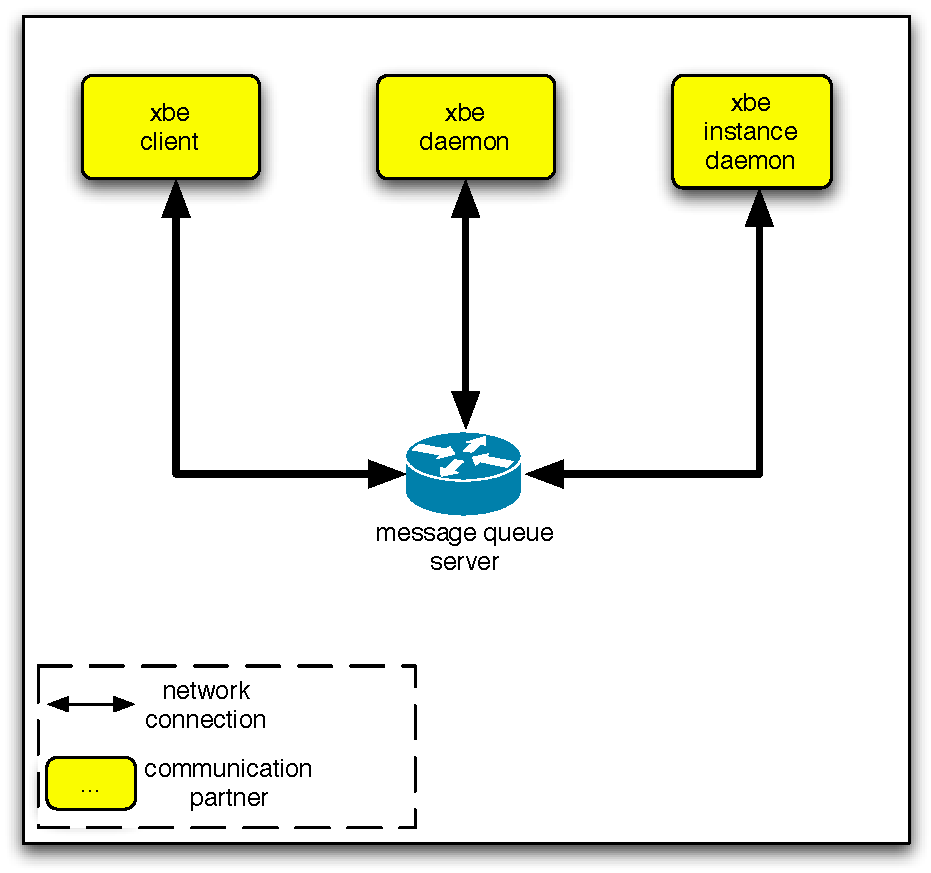
\includegraphics[scale=.75]{simple-network-topology}
  \caption[Network  Topology   (simple)]{The  simplest  network  topology,
    consisting of  only one Message  Queue Server and  three communication
    partners.}
  \label{fig:simple-net-top}
\end{figure}

\begin{figure}[ht]
  \centering
  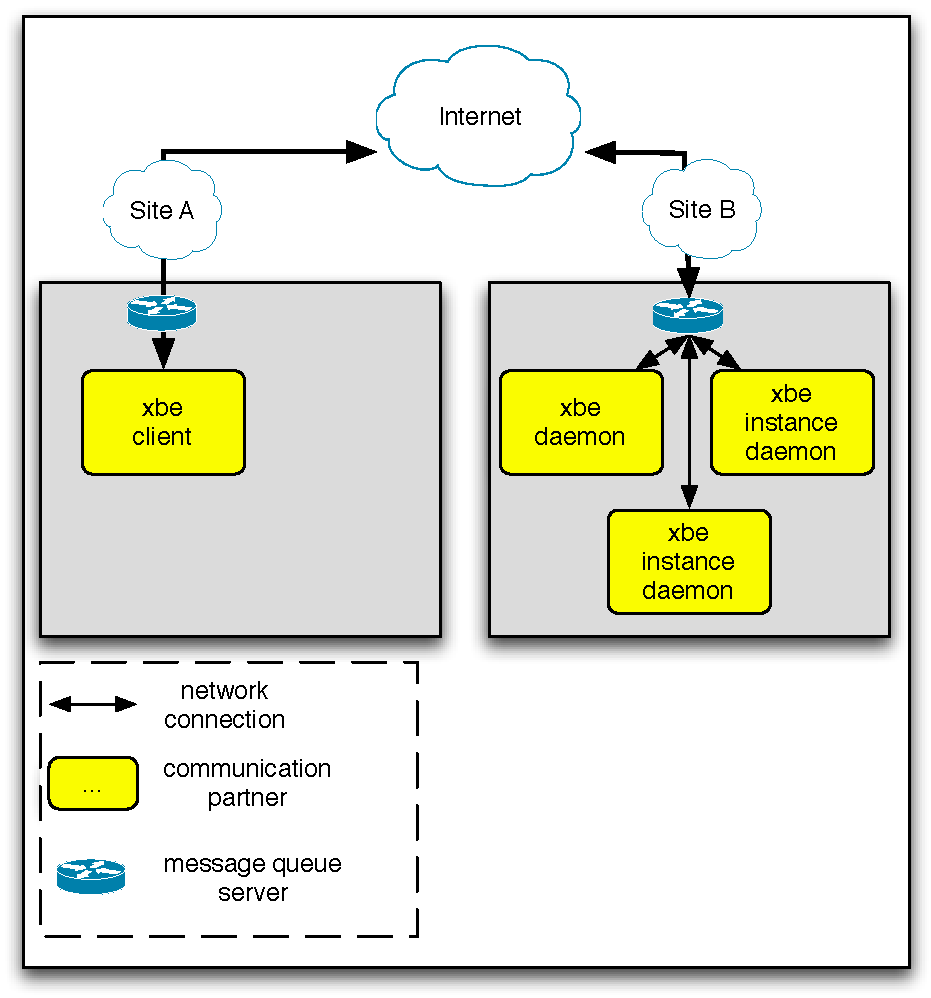
\includegraphics[scale=.75]{network-topology}
  \caption[Network  Topology]{TODO: fill me in}
  \label{fig:net-top}
\end{figure}

%%% Local Variables: 
%%% mode: latex
%%% TeX-master: "main"
%%% End: 
